\section{Virtualization}
\label{sec:virtual}
We strongly believe that a low cost of a device alone does not make it
attractive for inclusion in academic programmes.  There is a large
inertia to try out any new device.  A remotely operated laboratory
could be useful in this regard.  To try out such a device, a
prospective faculty instructor need not build any infrastructure.
They can remotely operate this device and also learn about it from the
educational material available.  If convinced, they can introduce them
in their curriculum.

Virtual labs are also the flavour of the day.  In this section, we
explain some of our experience in enabling the single board heater
system through the web.

% Virtual laboratory is one such network-based technique that allows
% remote monitoring and control of a real laboratory setup. In the
% pilot phase of the ongoing Virtual Labs project, funded by MHRD,
% Government of India, several virtual labs have been implemented and
% tested.  Remote access of single-board heater system, using LabVIEW,
% is one such initiative.

% LabVIEW, a proprietary software by National Instruments, is a
% graphical programming environment that facilitates measurement and
% testing, data storage and display, web publishing and also live data
% sharing using intuitive graphical icons and wires.

Web page to remotely access the LabVIEW front panel for collecting
step response data is shown in Fig. \ref{fig:rem-acc}. The available
knobs are used to vary fan speed and heater current. The resultant
temperature profile is observed on the same panel.  Other experiments
have also been implemented and tested for remote operation.  This
web-publishing feature facilitates only remote monitoring i.e. the
client can remotely vary the controller parameters with the
computation being done at the server end.

To overcome this, live data sharing across computers on intranet and
internet has been implemented and tested using NI DataSocket
technology. This interface is shown in Fig. \ref{fig:ds-inter}. With the
work still in progress, this feature explores the possibility of
controller located at the client end.

\begin{figure}
\centering
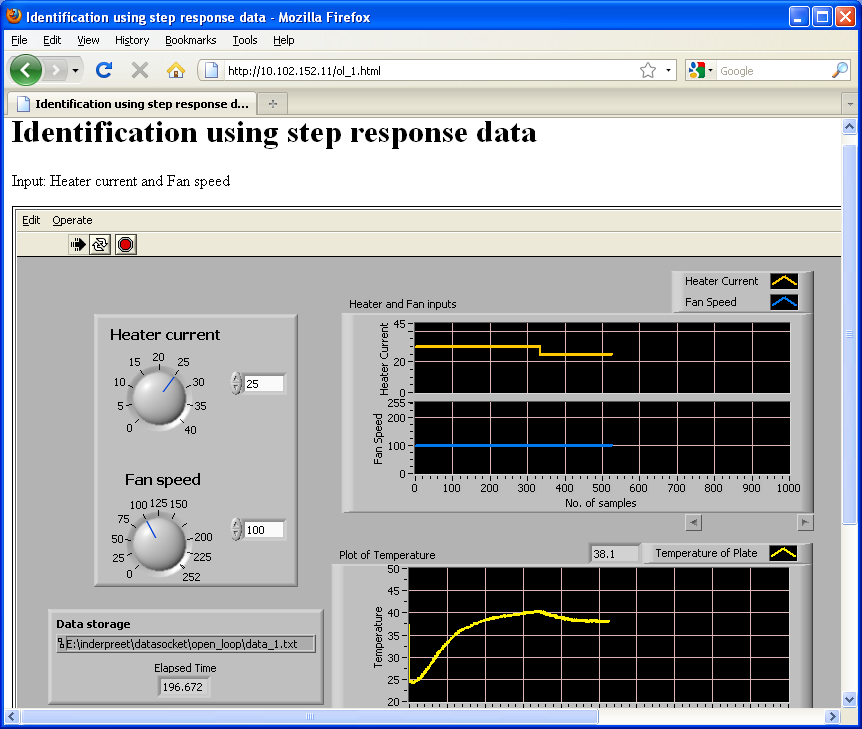
\includegraphics[width=0.9\linewidth]{lv-1}
\caption{Remote access of step response experiment}
\label{fig:rem-acc}
\end{figure}

\begin{figure}
\centering
\includegraphics[width=0.9\linewidth]{ds-1}
\caption{DataSocket technology for sharing live data}
\label{fig:ds-inter}
\end{figure}
